\documentclass[10pt]{ctexart}
\usepackage{hyperref}
\usepackage{graphicx}
\usepackage{subfig}
\usepackage{float}

\usepackage{listings}
\usepackage{minted}
\usepackage{color}
\definecolor{dkgreen}{rgb}{0,0.6,0}
\definecolor{gray}{rgb}{0.5,0.5,0.5}
\definecolor{mauve}{rgb}{0.58,0,0.82} % or use xcolor package to choose color
\lstset{frame=tb,
	language=Python,
	aboveskip=3mm,
	belowskip=3mm,
	showstringspaces=false,
	columns=flexible,
	basicstyle={\small\ttfamily},
	numbers=none,
	numberstyle=\tiny\color{gray},
	keywordstyle=\color{blue},
	commentstyle=\color{dkgreen},
	stringstyle=\color{mauve},
	breaklines=true,
	breakatwhitespace=true,
	tabsize=3
}

\title{PJ2 Report}
\author{Chen Hao 22307110062}

\begin{document}

\maketitle

\begin{abstract}
Implementation can be found in the codes at \url{https://github.com/Laplx/DLPJ} and will also be gradually explained in the following answers. The \textit{models} folder contains several model configurations, each corresponding to a specific question or modification and \textit{best.pth} is the final selected optimal version with an accuracy of \textbf{93.58\%} on the test set. 
\end{abstract}

\section{Task1: Train a Network on CIFAR-10}
\subsection{Basic Implementation}
我们使用了 Bottleneck 和 Resnet 结构,通过降低计算复杂度更高效的表达特征,同时残差连接缓解了梯度消失的问题。
\begin{lstlisting}
class Bottleneck(nn.Module):
	expansion = 4
	def __init__(self, in_planes, planes, stride=1):
		super(Bottleneck, self).__init__()
		self.conv1 = nn.Conv2d(in_planes, planes, kernel_size=1, bias=False)
		self.bn1 = nn.BatchNorm2d(planes)
		self.conv2 = nn.Conv2d(planes, planes, kernel_size=3, stride=stride, padding=1, bias=False)
		self.bn2 = nn.BatchNorm2d(planes)
		self.conv3 = nn.Conv2d(planes, planes * self.expansion, kernel_size=1, bias=False)
		self.bn3 = nn.BatchNorm2d(planes * self.expansion)
	
class ResNet(nn.Module):
	def __init__(self, block, num_blocks, num_classes=10):
		super(ResNet, self).__init__()
		self.in_planes = 64
		self.conv1 = nn.Conv2d(3, 64, kernel_size=3, stride=1, padding=1, bias=False)
		self.bn1 = nn.BatchNorm2d(64)
		self.layer1 = self._make_layer(block, 64, num_blocks[0], stride=1)
		self.layer2 = self._make_layer(block, 128, num_blocks[1], stride=2)
		self.layer3 = self._make_layer(block, 256, num_blocks[2], stride=2)
		self.layer4 = self._make_layer(block, 512, num_blocks[3], stride=2)
		self.linear = nn.Linear(512 * block.expansion, num_classes)
	
def Net():
	return ResNet(Bottleneck, [3, 4, 6, 3])
	
model = Net().to(device)
criterion = nn.CrossEntropyLoss()
optimizer = optim.Adam(model.parameters(), lr=0.001, weight_decay=1e-4)
scheduler = optim.lr_scheduler.CosineAnnealingLR(optimizer, T_max=100)
\end{lstlisting}

测试集准确率为 93.43\%。

\subsection{Different Configurations}
\begin{itemize}
	\item Different number of filters. 我们将全部通道数折半,同时训练 epoch 数由 100 缩减为 75,最终仍然几乎保持了测试集准确率(93.16\%)。
	
	\item Different loss functions. (保持了通道数折半,)将损失函数换为对标签经过光滑处理的交叉熵,它对除本标签外的其他标签均匀分配以 $\frac{\epsilon}{K-1}$ 的概率,其中 $K$ 为总标签数。或写为(其中 $CE$ 为标准交叉熵函数)
	
	$$
	\mathcal{L}=(1-\epsilon) \cdot \mathrm{CE}(y, p)+\epsilon \cdot \mathrm{CE}(u, p)
	$$
	
\begin{lstlisting}
class LabelSmoothingCrossEntropy(nn.Module):
	def __init__(self, smoothing=0.1):
		super(LabelSmoothingCrossEntropy, self).__init__()
		self.smoothing = smoothing
		self.confidence = 1.0 - smoothing
		
	def forward(self, output, target):
		log_probs = F.log_softmax(output, dim=-1)
		n_classes = output.size(-1)
		true_dist = torch.zeros_like(log_probs)
		true_dist.fill_(self.smoothing / (n_classes - 1))
		true_dist.scatter_(1, target.data.unsqueeze(1), self.confidence)
		return torch.mean(torch.sum(-true_dist * log_probs, dim=-1))
\end{lstlisting}
	
	测试集准确率达到了更优的水平,为 93.52\%;猜测软化真实标签可能缓解了模型对硬标签的过拟合,提升泛化能力。
	
	\item Different activations. 我们将各层的激活函数由 RELU 换为了更为光滑的 GELU。(且此时可以发现 epoch 基本只需 20 - 30 个即已基本收敛到最优。)测试集准确率为 93.58\%。激活函数本身形式没有造成特别大的改进或退化的影响。
	
	\item Different optimizers. 
	
\begin{lstlisting}
optimizer = optim.AdamW(model.parameters(), lr=0.001, weight_decay=0.01)
scheduler = optim.lr_scheduler.OneCycleLR(optimizer, max_lr=0.003, total_steps=100 * len(trainloader), pct_start=0.3)
\end{lstlisting}
	
	测试集准确率反而下降到了 92.14\%;可能是自适应学习率在数据噪声较大时梯度估计不稳定,或较高的初始学习率超出模型容忍范围。
	
\end{itemize}

\subsection{Network Visualization}
\begin{itemize}
	\item Filters. 我们绘制了第一层各卷积核的权重图(按最大最小归一,可视化具体实现见代码)。
	\begin{figure}[H]
		\centering
		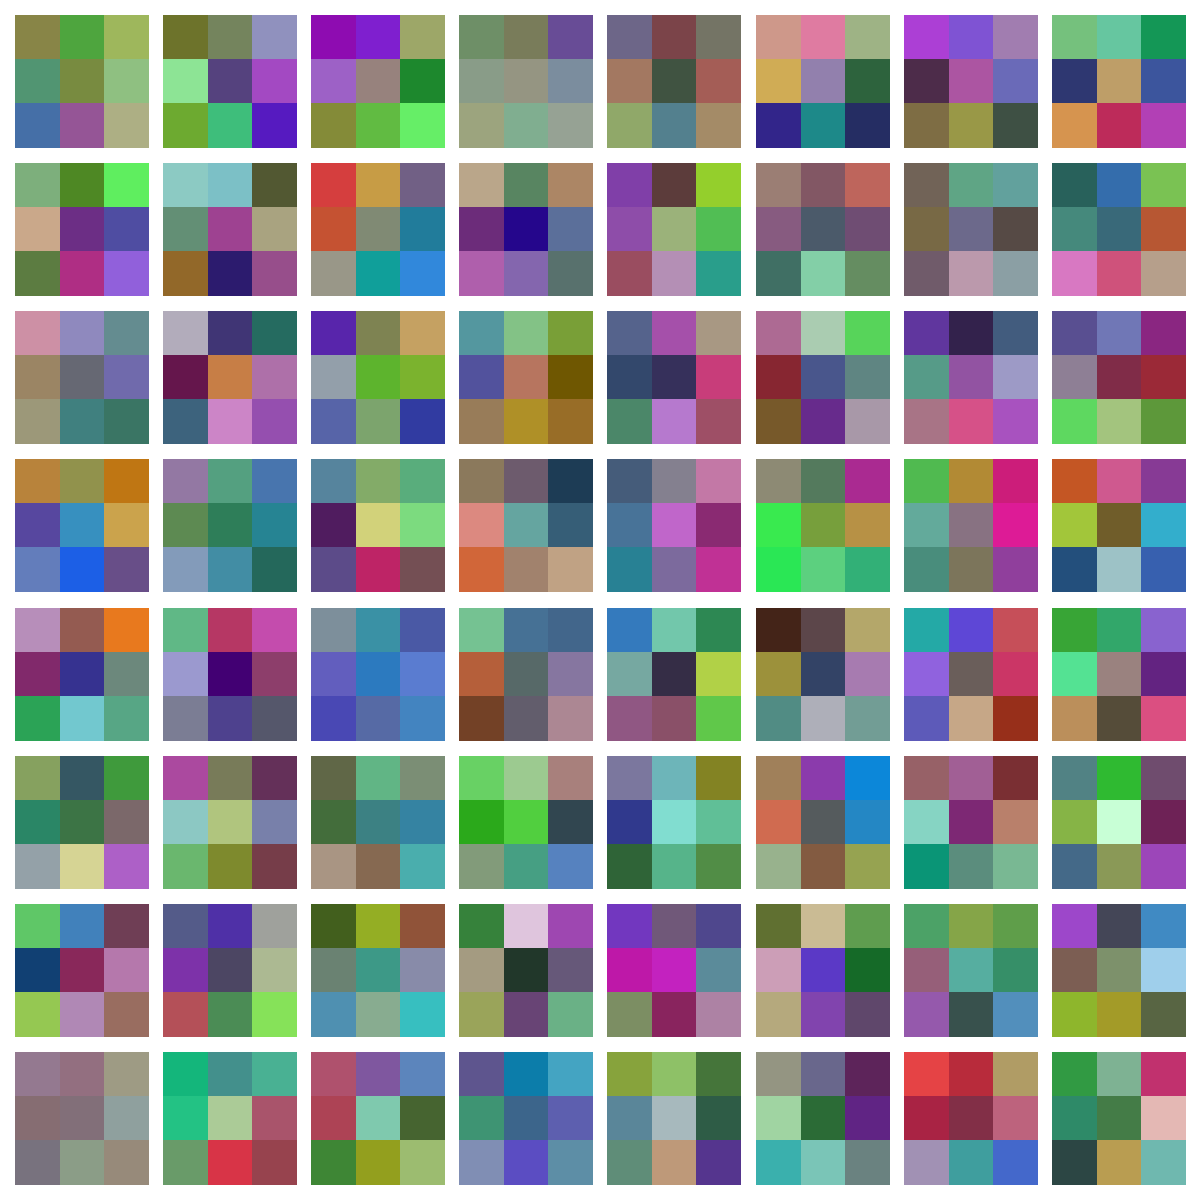
\includegraphics[width=0.6\linewidth]{filters_conv1.png}
		\caption{Filters of conv1}
	\end{figure}
	
	\item Loss landscape. 我们通过在模型参数空间的两个随机方向上扰动参数并计算损失值,生成3D图形展示损失函数的变化趋势;可以看到虽然表面凹凸非常不平,但是整体又呈现显著的一个下降方向,这显示了神经网络优化问题的共性。
	
	\begin{figure}[hb]
		\centering
		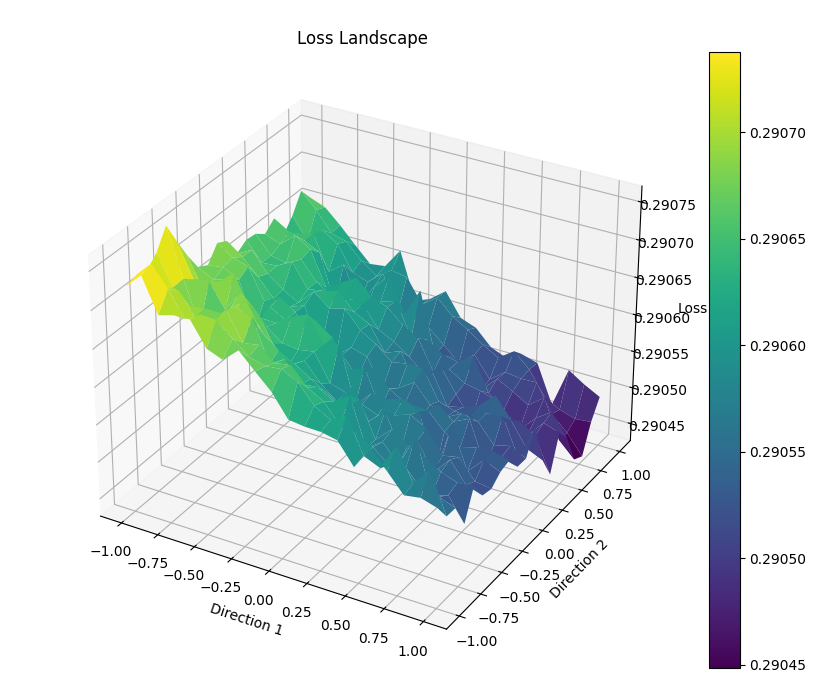
\includegraphics[width=0.7\linewidth]{loss_landscape.png}
		\caption{}
	\end{figure}
	
	\item Network interpretation. ​​我们通过 Grad-CAM(梯度加权类激活映射)​​的可视化,提取模型最后一个卷积层的特征和梯度,生成热力图来展示输入图像中对分类决策最重要的区域。可以看到网络学习明显到了各类别物体的所在和判断,并且深色处较为可信的聚焦在特征部位。
	
	\begin{figure}[H]
		\centering
		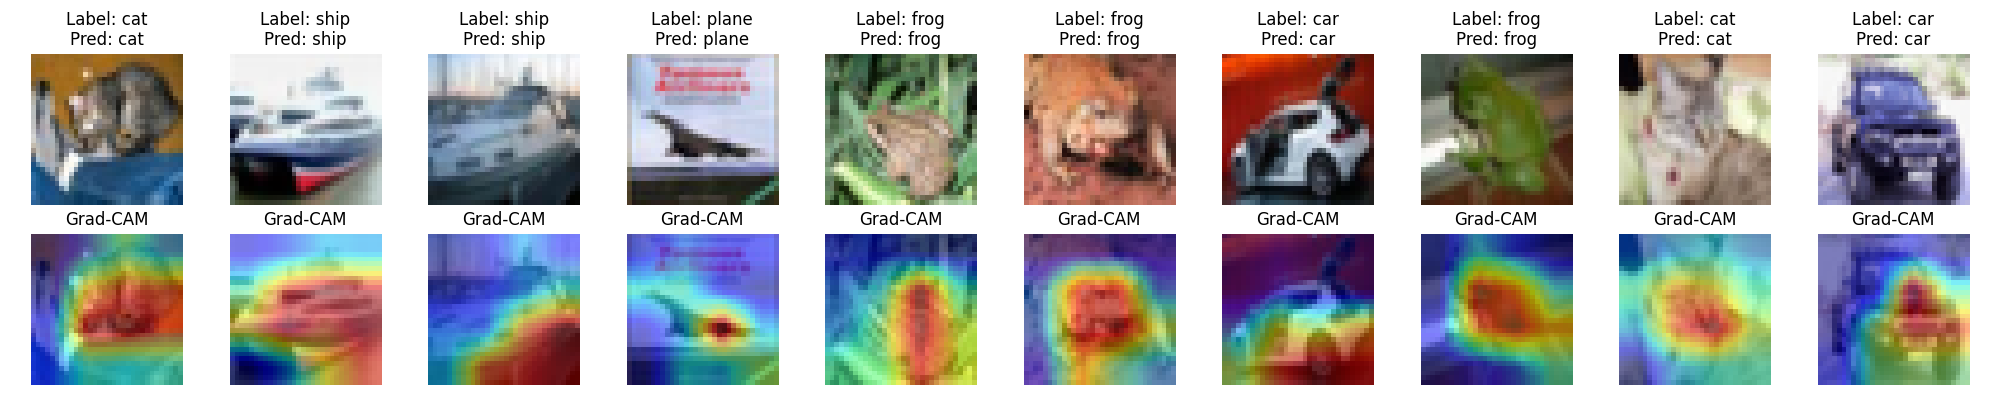
\includegraphics[width=1.1\linewidth]{grad_cam.png}
		\caption{Grad-CAM visualization}
	\end{figure}
\end{itemize}                        


\section{Task2: Batch Normalization}
\subsection{VGG-A with and without BN}
实现了 VGG-A 的归一化层之后我们可以画出两边训练的损失图景作比较。

\begin{figure}[h]
	\centering
	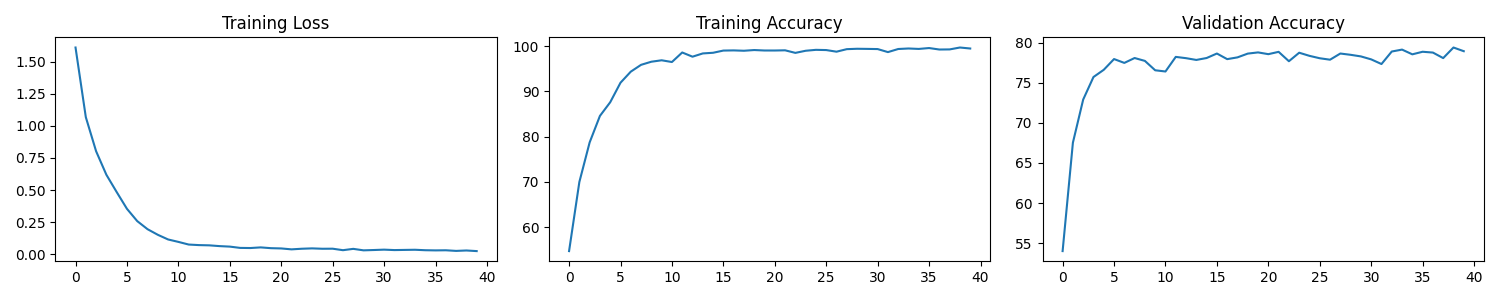
\includegraphics[width=0.9\linewidth]{training_curve_epoch_40.png}
	\caption{Training curve of VGG-A without BN at epoch 40}
\end{figure}

\begin{figure}[h]
	\centering
	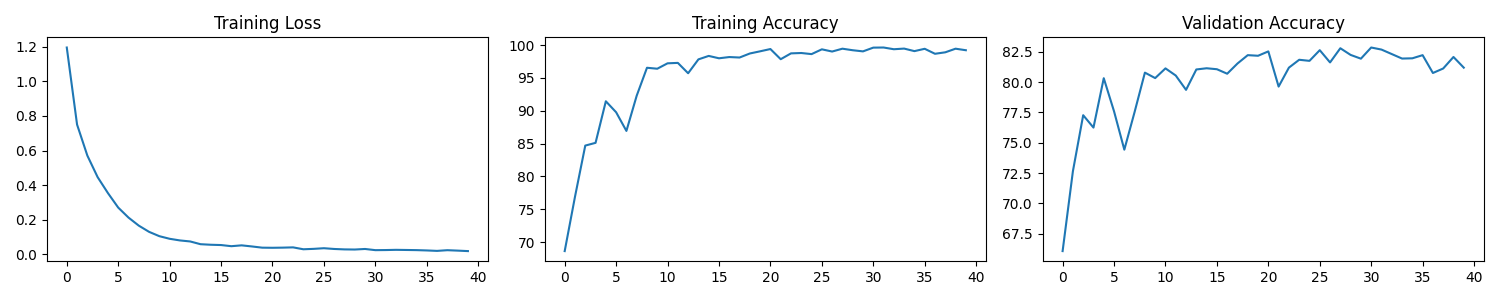
\includegraphics[width=0.9\linewidth]{training_curve_bn_epoch_40.png}
	\caption{Training curve of VGG-A with BN at epoch 40}
\end{figure}

\begin{figure}[h]
	\centering
	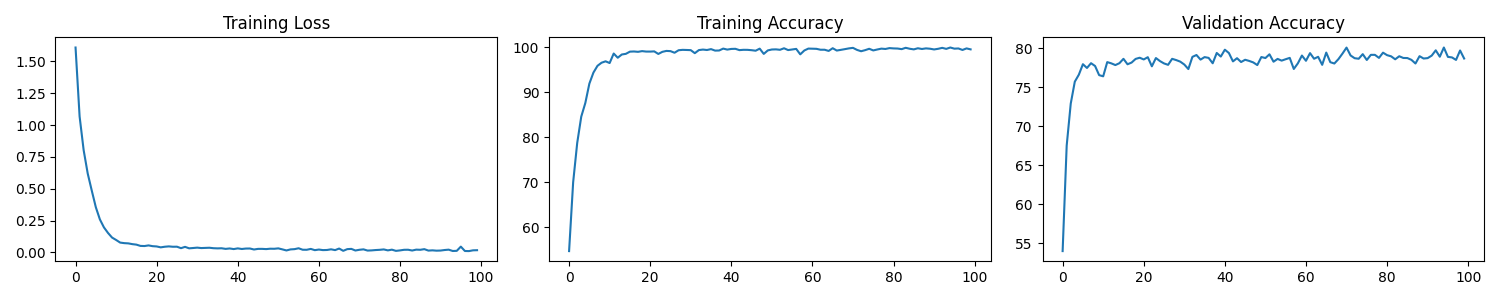
\includegraphics[width=0.9\linewidth]{training_curve_epoch_100.png}
	\caption{Training curve of VGG-A with BN at epoch 100}
\end{figure}

值得注意的是,尽管在后期包括最终的准确率上带归一层的网络胜出;但同样在第 40 个 epoch,有归一化层的网络反而情况不如没有的理想,一个猜测可能是归一层导致网络携带了更多的参数量,同时本身网络参数量可能已经略微过度,所以在最初相同批次下收敛速度不快。

\subsection{Loss Landscape}
遵照文件里的指示,我们选取了 $[1e-3, 2e-3, 1e-4, 5e-4]$ 几个学习率分别对两种网络进行训练,以画出最终的损失景观的对比图。

\begin{figure}[h]
	\centering
	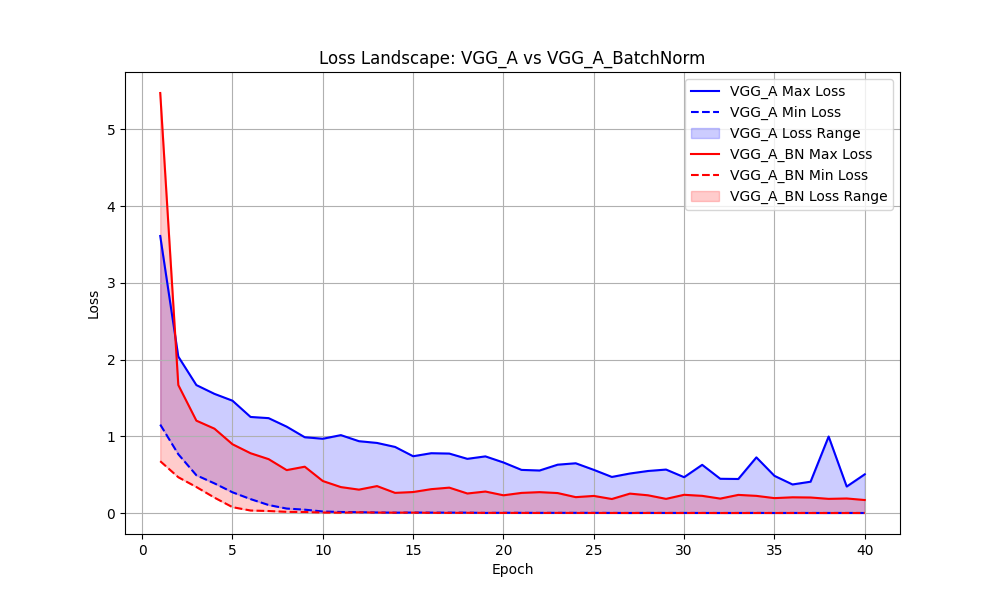
\includegraphics[width=0.7\linewidth]{loss_landscape_bn.png}
	\caption{}
\end{figure}

可以看出归一层的一个显著作用是控制了损失值的波动;但这里后段下界基本接近于 0 可能是由于网络拟合能力已经基本超出了 32 * 32 所需要的处理能力。

\end{document}
